
\begin{SCfigure*}
	\centering
	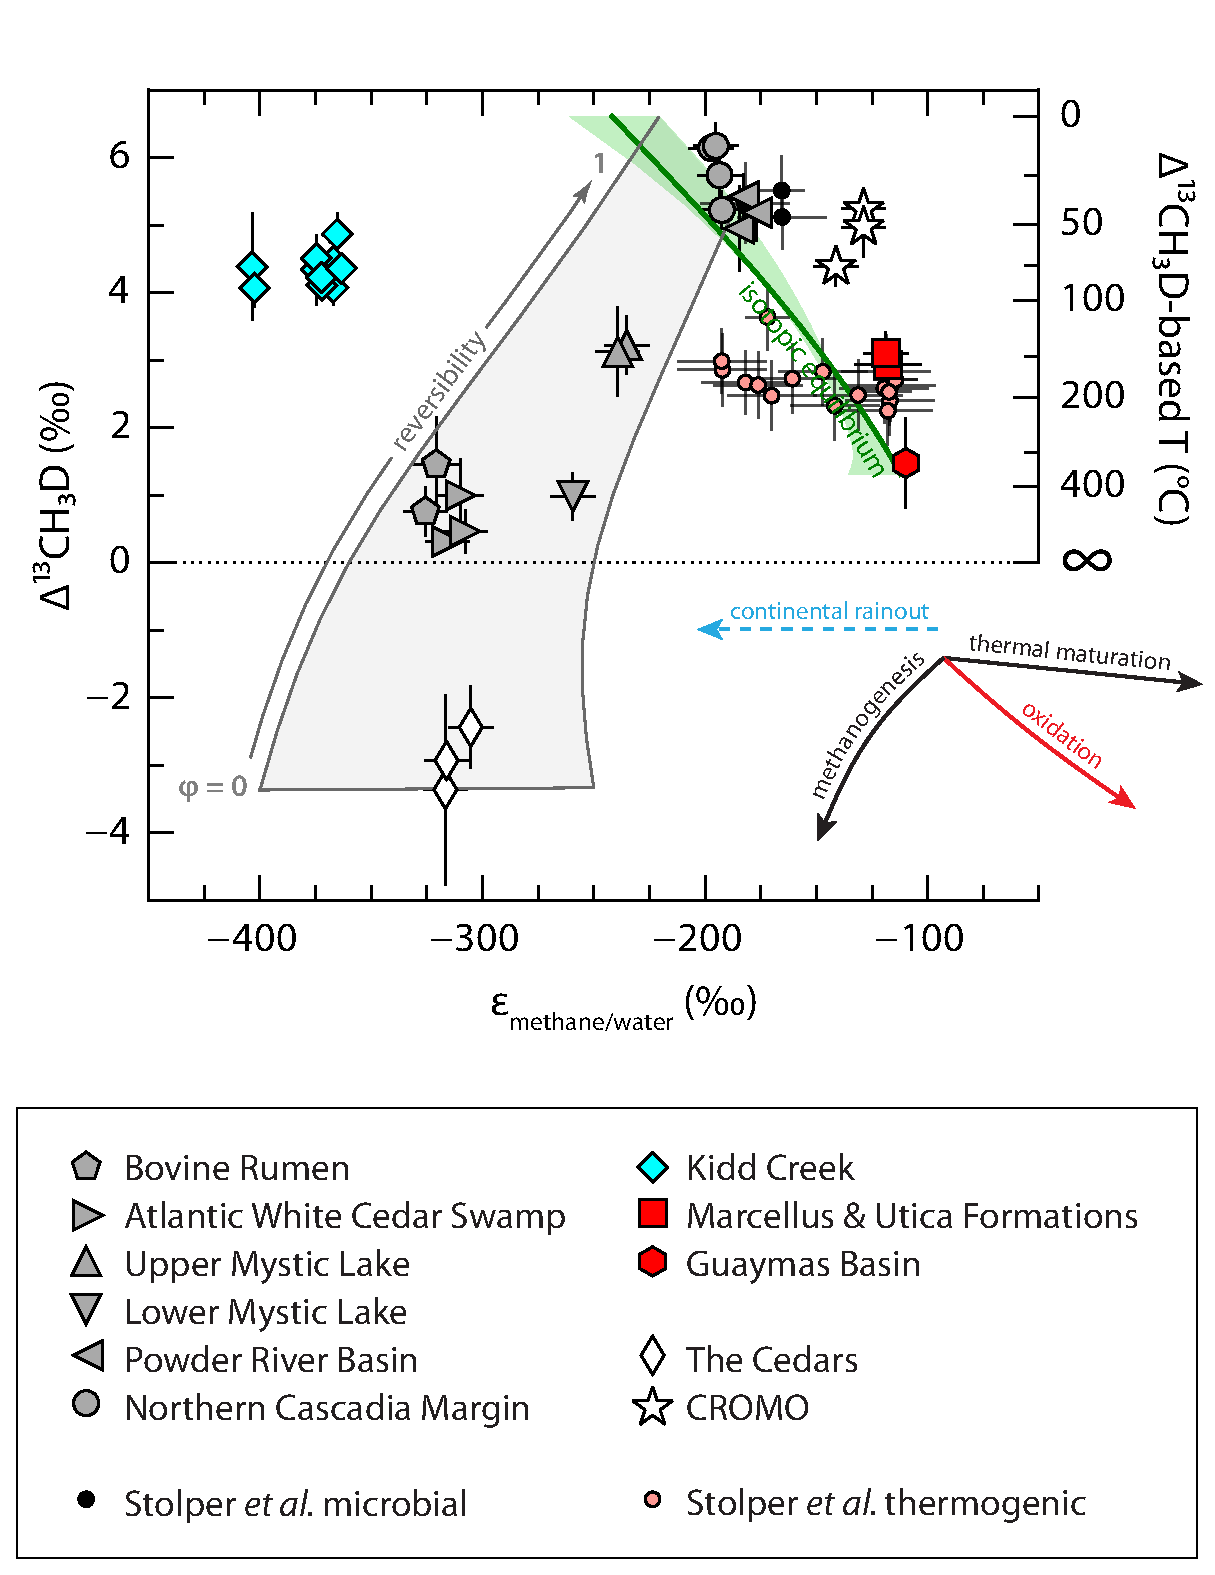
\includegraphics[width=0.57\textwidth]{figures/Fig5.2.pdf}
	\captionsetup{format=myformat}	% hrule beneath caption
	\caption[A survey of \textsuperscript{13}CH\textsubscript{3}D in the environment]{A survey of \textsuperscript{13}CH\textsubscript{3}D in
		the environment. This figure is the same as \autoref{fig:2:2}, with
		the addition of schematic vectors showing basic controls on the isotopic
		signatures of CH\textsubscript{4}, and data from \textcite{Stolper++_2014_S}.
		The position of their data along the \emph{x}-axis was calculated from
		estimated δD of formation waters, and for the \emph{y}-axis,
		Δ\textsubscript{18} values were converted to
		Δ\textsuperscript{13}CH\textsubscript{3}D by assuming equilibrium and
		applying the conversion shown in \mrefs[A]{Fig.}{fig:C:2}.}
	\label{fig:5:2}
\end{SCfigure*}